\section{Теория}

\begin{frame}
    \frametitle{Совместные задания для групп}
    \centering
    \begin{figure}
        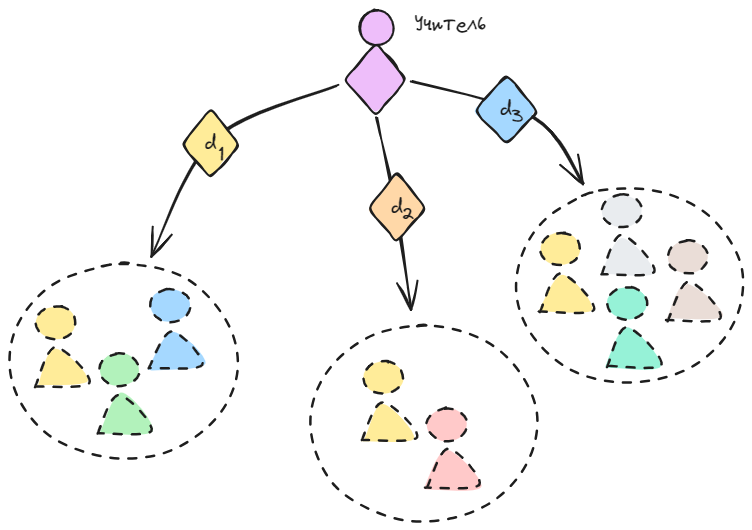
\includegraphics[width=0.8\linewidth]{assets/setting/groups.excalidraw.png}
    \end{figure}
\end{frame}

\begin{frame}
    \frametitle{Описание}
    \begin{block}{Постановка}
        Учащиеся объединяются в $k$ групп. Каждой группе $i$ предлагается задача сложности $d_i$. 
    \end{block}

    \begin{exampleblock}{Преимущества}
        \begin{itemize}
            \item оптимальное число заданий к проверке
            \item обучение командной работе
            \item \textbf{применимость адаптивного обучения} 
        \end{itemize}
    \end{exampleblock}

    \begin{alertblock}{Проблемы}
        \begin{itemize}
            \item неравномерное распределение нагрузки в группе
            \item неясность в выборе сложности задания
        \end{itemize}
    \end{alertblock}
\end{frame}

\begin{frame}
    \frametitle{Алгоритм Роббинса-Монро для функций многих переменных}
    Обобщение алгоритма для случая многомерной функции отклика 
    задаёт условия на параметры схемы. \footnote{Xiong, Cui, and Jin Xu. "Efficient Robbins–Monro procedure for multivariate binary data."}
    \begin{block}{Алгоритм Роббинса-Монро для случая многих переменных}
        Пусть $\vec{x}$ - вектор бернулевских случайных величин с параметрами $\vec{s}=f(\vec{d})$, где $f(\vec{x})$ - выпуклая.
        Тогда cхема пересчета $d_t=\vec{x}_t + A^{(t)} (s - \vec{x}_t)$ с шагами $A^{(t)}$ удовлетворяющих условиям:
        $\forall t,j \rightarrow a_{jj}^{(t)} >0,
        \sum^{\infty}_{t=1} a_{jj}^{(t)} = \infty,
         \sum_{n=1}^\infty (a^{(t)}_{jj})^2 < \infty$
        сходится по вероятности к целевому значению $\vec{s}^*$
    \end{block}
\end{frame}


\begin{frame}
    \frametitle{Супераддитивность в групповом образовании}
    \begin{block}{Эффективность совместногого обучения}
        Считаем, что эффективность учащихся задается как гауссова случайная величина$$
            \vec{x} \sim \mathcal{N}(\vec{\mu}, \Sigma).
        $$
        Матрица ковариации $\Sigma$ задает эффективность командной работы
    \end{block}
    \begin{block}{Супераддитивность}
        Супераддитивной называется функция $f$ для которой
        \begin{equation}
            \forall x, y, x+y \in \text{dom}(f) \rightarrow f(x+y) \ge f(x) +f(y) 
        \end{equation}
    \end{block}

    \begin{block}{Функции к изучению}
        \begin{itemize}
            \item min-sum $\sum_{i} min([\vec{x}]_i,s^*)$, гдe $s^*$ - порог отсечки
            \item max-mean $N \cdot \bar{x} + \max_i(\vec{x} - \bar{x})$
            \item квадратичная форма $\vec{x}^T A \vec{x}$
        \end{itemize}
    \end{block}
\end{frame}